\begin{displayquote}
	\textsf{After the validation of numerical and parallel performances of $m$-UCGLE, a major difficulty to profit from UC methods including $m$-UCGLE is to implement the manager engine which can well handle their fault tolerance, load balance, asynchronous communication of signals, arrays and vectors, the management of different computing units such as GPUs, etc. In Chapter \ref{UCGLE for Linear Systems with Multiple Right-hand-sides}, we tried to give a naive implementation of an engine to support the management computing components on the homogeneous/heterogeneous platforms based on MPI\_SPAWN and MPI non-blocking sending and receiving functionalities. The stability of this implementation of the engine cannot always be guaranteed. Thus we are also thinking about to select the suitable workflow/task based environments to manage all these aspects in the UC approach. YML\footnote{http://yml.prism.uvsq.fr/} is a good candidate, which is a workflow environment to provide the definition of the parallel application independently from the underlying middleware used. The special middleware and workflow scheduler provided by YML allows defining the dependencies of tasks and data on the supercomputers \cite{delannoyyml}. YML, including its interfaces and compiler to various programming languages and libraries, will facilitate the implementation of UC based methods with different numerical components. In this chapter, firstly we give a quick summary of the YML framework and then analyze the limitations of existing YML implementation for UC approach. In the end, we propose related solutions.}
\end{displayquote}

\vspace{0.6in}


\section{YML Framework}

YML is a workflow environment dedicated to the execution of parallel and distributed applications on different Grid platforms and supercomputers. The YML framework enables the description of the complex parallel application based on the tasks. The task-based application written based on YML language can be executed on several runtime systems or middleware without changes. YML is a software layer between the end-user and the runtime system of a supercomputer and/or the middleware of a distributed system, which is in charge of communication. 

\subsection{Structure of YML}

YML is composed of three main parts: an IDL (Interface Description Language), a kernel and a backend allowing interactions with the runtime system or middleware. As shown in Fig. \ref{yml-arch}, the kernel of YML consists of a high-level workflow language, a just-in-time scheduler and a system of service integration. The high-level language (YvetteML) which is XML-based permits the description of the graph of application with dependencies or communications. The language integrates the ability to describe computation and their workflow on the same time. This language provides a way to specify the communication between components during the execution of the application. The graph can contain parallel and sequential sections and standard construction of most languages including branching, exceptions, and loops. The graph language describes the dependencies between the components during the execution by the notion of events. The compiler translates the graph of components of applications in an internal representation containing a set of components calls. The scheduler manages application execution and acts as a client for the underlying runtime system accurately requiring computing resources. During the execution, the scheduler detects tasks ready for execution and solves their dependencies at runtime. Each scheduling step may generate different types of tasks (parallel or serial), which are supported dedicated middleware and backends. With the component-oriented design of YML, a service in YML can be any kind of components such as a library, a data repository, or a catalog of binary components. The computation components can be written in different programming languages like C, C++ and XcalableMP. 

\subsection{YML Design}

The aim of YML is to provide users with an easy-of-use method to run parallel applications on different Grid platforms and supercomputers. The framework can be divided into three parts which are the \textit{end-users interface}, \textit{frontend}, and \textit{backend}. The end-users interface is used to provide an intuitive way to submit their applications, which are described using a workflow language YvetteML. Frontend is the main part of YML which includes a compiler, scheduler, data repository, abstract and implementation components (shown as Fig. \ref{yml-arch}). The backend is the part to connect different Grid, P2P and cluster middlewares.

\begin{figure}[htbp]
	\centering
	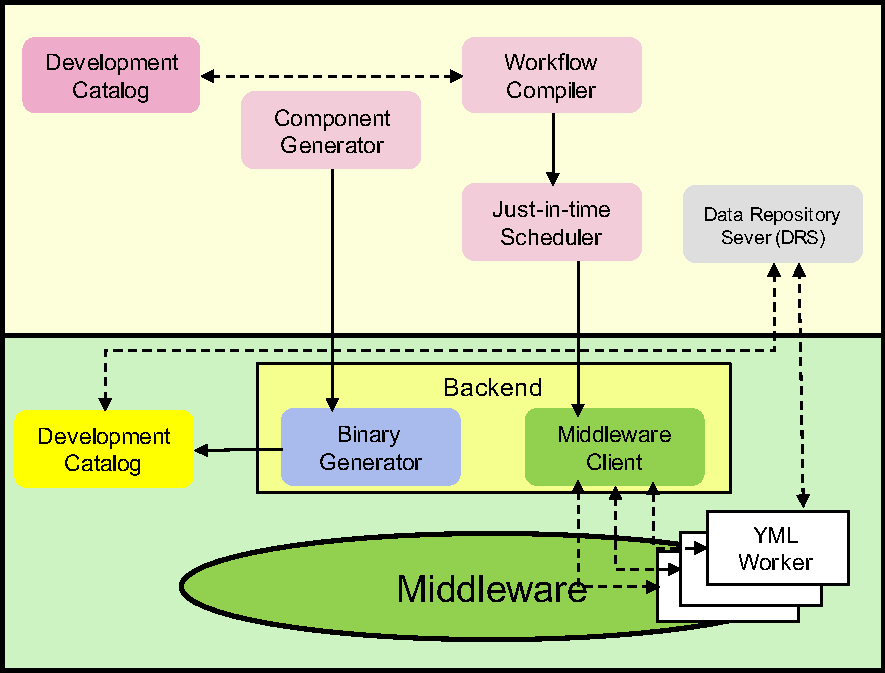
\includegraphics[width=.92\linewidth]{fig/yml-arch.pdf}
	\caption{YML Architecture.}
	\label{yml-arch}
\end{figure}

The development of a YML application is based on the components approach, and then we will discuss the three kinds of components in detail.

\begin{itemize}
	\item \textbf{Abstract component} defines the communication interface with the other components. This definition gives the name, and the communication channels correspond to a data input, data output or both and are typed. This component is used in the code generation step and to create the graph.
	
	\item \textbf{Implementation component} is the implementation of an abstract component. It describes computations through YvetteML language. The implementation is done by using common languages like C or C++. They can have several implementations for the same abstract component.
	
	\item \textbf{Graph component} carries a graph expressed in YvetteML instead of a description of computation. It provides the parallel and sequential parts of an application and the synchronization events between dependent components. It is a straightforward way for scientific researchers to develop their application.
\end{itemize}

Moreover, those three components are independent of middleware, which can be reused on various platforms. In order to run an application on other computing environments with a different middleware, the user needs to compile each component for the selected middleware.  YML eases components creation. Existing code can be reused by importing libraries as some new components without any adaptation. Those components are called by the application when computational tasks have to be started. Moreover, the notions of abstract and implementation descriptions of components bring three interesting features for the scheduler that can be included in the framework.

\begin{itemize}
	\item \textbf{data migration} can be easily quantified at the start and at the end of the application thanks to the abstract definition.
	\item \textbf{data used} by a component is clearly defined in the abstract and implementation definitions, therefore this can be used in a checkpointing feature to move a component from a node to an other.
	\item \textbf{computation time} of a component can be evaluated thanks to the implementation definition.
\end{itemize}

The use of Data Repository Servers hides the data migrations to the developer and ensure that necessary data are always available to all components of the application.

\subsection{Workflow and Dataflow}

The workflow programming environment YML facilitates the expression of parallelism for the user, which is able to implement the applications in a way very close to the algorithms. YvetteML, the high-level language provided by YML, is able to describe easily the complex workflow of applications. The \textit{Abstract} provides the interface of components including the input and output data. When a graph of tasks is constructed, the dataflow can be deduced by the input/output data types defined in the \textit{Abstract} of components. As shown in Fig. \ref{fig:yml-dataflow}, YML enables the optimization combining two aspects:

\begin{itemize}
	\item workflow;
	\item dataflow
\end{itemize}

\begin{figure}[htbp]
	\centering
	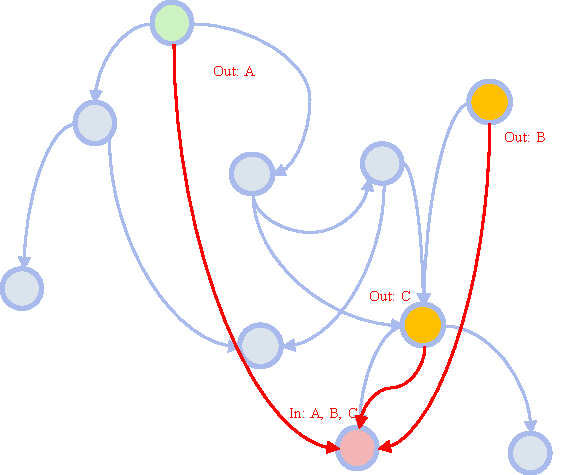
\includegraphics[width=.72\linewidth]{fig/dataflow.pdf}
	\caption{YML workflow and dataflow.}
	\label{fig:yml-dataflow}
\end{figure}

\subsection{YvetteML Language}

The YvetteML language provides different features for creating applications. These features are described as below:

\begin{itemize}
	\item \textbf{Parallel Section:} they are used to explicitly define sections which will be executed in parallel. The formule of this operation is given as: \textit{par section 1 // ... // section N endpar};
	\item \textbf{Sequential loop:} they are loops with iterators, which are executed sequentially. The formule of this operation is given as: \textit{seq (i:=begin;end) do ... enddo};
	\item \textbf{Parallel loop:} they are loops with iterators, which are executed in parallel. The formule of this operation is given as: \textit{par (i:=begin;end) do ... enddo};
	\item \textbf{Conditional structure:} they are the condition structure to control the execution of tasks by the condition. The formule of this operation is given as: \textit{if (condition) then ... else ... endif};
	\item \textbf{Synchronization:} The formule of this operation is given as: \textit{wait(event) / notify(event)};
	\item \textbf{Component calls:} the role of component calls is to submit a new task to the Local Ressource Manger providing the name of the component defined earlier and the different input parameters. The formule of this operation is given as: \textit{compute NameOfComponent(args,...,...)}.
\end{itemize}

\subsection{YML Scheduler}

In computing, scheduling is a method in which work specified in some way is assigned to resources that complete work. The scheduler performs scheduling activities, and the scheduler is usually implemented to keep all computing resources busy. A scheduler may aim to one of many goals, maximizing throughput (the total amount of work completed per time unit), minimizing response time (time from work becoming enabled until the first point it begins executing resources), minimizing latency (the time between work becoming enabled and its subsequent completion) or maximizing fairness (equals CPU time to each process, or more generally appropriate times according to the priority and workload of each process).

\subsubsection{Scheduler Architecture}

For the scheduling, the YML environment is defined in two parts:

\begin{enumerate}[label=(\arabic*)]
	\item The first part is what we call the \textbf{frontend}. Its mission is to analyze the application code written by YvetteML and dispatch the tasks for the backend and middlewares.
	\item  The second part is the \textbf{backend}.  It deals  with the distribution of tasks onto different computing units.
\end{enumerate}

\subsubsection{Frontend}

Now we are talking about the scheduler of YML. It is responsible for reading the dependency graph by compiling the graph of application. This graph contains all inner-steps dependencies. The scheduler is closely linked to the worker component. Indeed the worker component is a component responsible for the execution of a service. Services represent computations needed for the realization of a workflow process, the execution of a service can be decomposed in the following steps: 

\begin{enumerate}[label=(\arabic*)]
	
	\item  When the worker component is started, it first analyzes a work description. This work description contains all the information needed to execute the service. It consists of a list of resources to retrieve from the data repository component, the parameter of the service as well as the destination of the results. The resources retrieved are the service and its input. The service is then executed. 
	
	\item  It generates a set of results as well as some meta-information such as the status reported by the service, the list of results produced and a trace of the execution of a service. 
	
	\item The information is published to the data repository component together with the results of the service. 
	
	\item  The worker finally cleans up the peer and finishes its execution. The workflow scheduler component is responsible for executing workflow processes. 
\end{enumerate}

As shown by Algorithm \ref{alg:yml-scheduler}, the scheduler executes two main operations sequentially. Firstly, it schedules the execution of workflow by solving the dependencies among its activities and submit them to the backend. The generation of new tasks is following a new schedule rule updated from the scheduler.  The second operation is the monitoring of the task currently being executed. Once tasks have started their execution, the scheduler of the application regularly checks if new works have entered the finished state. The scheduler interacts with the backend layer through the data repository and backend components. Every time a work status changed to ready, the scheduler prepares the execution of a service by creating a script describing the work. This script is processed by the worker component of the backend layer. In the meantime, the work channels are stored in an archive in order to be easily exchanged between the data repository and the worker. If a task is finished, it will be deleted, and its status will be updated to the scheduler. Besides, the scheduler is able to manage the execution errors of computing components. 

\begin{algorithm}[t]{}
	\caption{YML Scheduler}   
	\label{alg:yml-scheduler}   
	\begin{algorithmic}[1]
		\While {\textit{status} == EXECUTING}
			\While {\textit{task} == \textit{finished}}
				\State ++\textit{taskFinished}
				\State delete(\textit{task})
			\EndWhile
			\State \textit{UpdateStatus}
			\If{\textit{status}==ERROR}
				\State continue \Comment{Task terminates with error, execution stopped}
			\EndIf 
			\State \textit{UpdateSchedulingRule}
			\While {(\textit{task} = \textit{nextTaskReady}) !=0}
				\State ++\textit{taskSubmitted}
				\State \textit{queue(task)}
			\EndWhile
			\If {!\textit{SchedulingPendingTask}}
				\State break \Comment{Execution finished with error}
			\EndIf
			\State \textit{updateStatus}
		\EndWhile
		\State \textit{finalizeExecution}
	\end{algorithmic}  
\end{algorithm}

\subsubsection{Backend}

The backend component is responsible for the interaction with the resource scheduler service of the middleware. It translates the abstract work description composing a workflow into requests to the resource scheduler of a middleware. Each middleware has its own backend component. The backend component acts as a client of the middleware. The abstract work request which is processed by the backend component leads to the execution of a worker component on a peer selected by the middleware resource scheduler. The worker component analyzes the work description and is responsible for its execution. Its means the acquisition of the concrete service used to do the computation and the data required for the computation. Then, the worker executes the concrete service corresponding to the work. And finally, the worker as well as the kernel layer interact with the data repository component. This component is responsible for the acquisition as well as the publishing of data in the workflow environment. The model thus defines two operations:

\begin{itemize}
	\item \textbf{put}: this operation is used to publish data within a data repository or a network of repositories. Publishing data is similar to write operation on a memory area;
	\item \textbf{get}: this operation is used to acquire data stored in a data repository. Acquiring a data is similar to read operation on a memory area.
\end{itemize}

The backend component allows the submission of asynchronous invocation of applications on peers. The resource scheduler selects arbitrary a peer and assigns it to the execution of the request. The content of the request varies significantly from one middleware to another. The backend component translates YML service execution into requests understandable by the resource scheduler of the middleware currently used. A backend component maintains a list of active requests and a list of finished requests. The polling of the middleware allows the backend to move requests from the active queue to the queue of finishde requests. In YML, a request consists in the execution of the worker component by a peer, thus the backend allows YML to ask the middleware to execute many instances of the YML worker and to be notified when one terminates. 


\subsection{Multi-level Programming Paradigm: YML/XMP}

A multi-level programming model  on the supercomputing systems is established by combing YML and XMP. YML/XMP programming model requires a specific middleware \textit{OmniRPC-MPI}. The multi-level parallelism including:

\begin{itemize}
	\item High level: communication inter nodes/group of nodes
	\begin{itemize}
		\item YML - coarse grain parallelism - asynchronous communication
	\end{itemize}
	\item Low level: group of nodes / cores
	\begin{itemize}
		\item PGAS language XMP programming with pragma
	\end{itemize}
\end{itemize}

The multi-level programming paradigm YML/XMP is supported by the\textit{OmniRPC-MPI} middleware. \textit{OmniRPC} is a thread-safe remote procedure call (RPC) system, based on Ninf, for cluster and grid environment. It supports typical master/worker grid applications. Workers are listed in an XML file named as the host file. For each host, the maximum number of job, the path of OmniRPC, the connection protocol (ssh, rsh) and the user can be defined.

An OmniRPC application contains a client program which calls remote procedures through the OmniRPC agent. Remote libraries which contain the remote procedures are executed by the remote computation hosts. There are implemented like an executable program which contains a network stub routine as its main routine. The declaration of a remote function of the remote library is defined by an interface in the Ninf IDL. The implementation can be written in familiar scientific computation language like FORTRAN, C or C++. There are two versions of OmniRPC. One is for the grid computing and distributed architecture of large numbers of computers and the other for supercomputer (OmniRPC-MPI).  The scheduler of OmniRPC is simple. It is just a classic Round-Robin scheduling algorithm.  As the term is generally used, time sliced are assigned to each process in equal portions and circular order, handling all processes without priority (also known as the cyclic executive). Round-Robin scheduling is easy to implement and starvation-free.

\subsection{YML Example}

In this section, we give an example to understand the grammar and implementation of YML. The workflow of this example is given as Fig. \ref{fig:sum_workflow}. Its scenario is: firstly two seperate sum operations of four given floating numbers are executed, which result in two different floating numbers, these two numbers are added together to output the final results.
 
\begin{figure*}[htbp]
	\centering
	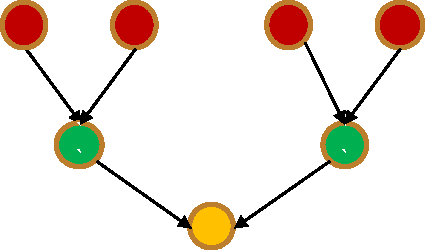
\includegraphics[width=3.in]{fig/sum_workflow.pdf}
	\caption{Workflow of Sum Application.}
	\label{fig:sum_workflow}
\end{figure*}

\subsubsection{Abstract}

The \textit{Abstract} defines the communication interface with the other components. This definition gives the name, and the communication channels correspond to a data input, data output or both and are typed. This component is used in the code generation step and to create the graph. As shown in the Listing \ref{abstr}, the \textit{sum} operation requires two input parameters $a$ and $b$, and an output parameter $res$. These three parameters are all of scalar type \textit{real}. 

\begin{listing}
\begin{minted}
[
frame=lines,
framesep=2mm,
baselinestretch=1.2,
bgcolor=gray!10,
%fontsize=\footnotesize,
%linenos
escapeinside=!!
]
	{xml}
<?xml version="1.0" encoding="utf-8"?>
<component type="abstract" name="test_abstract"
description="sum of two doubles">
  <param type="real" mode="out" name="res" />
  <param type="real" mode="in" name="a" />
  <param type="real" mode="in" name="b" />
</component>
\end{minted}
\caption{\textit{Abstract Component} Example}
\label{abstr}
\end{listing}

\subsubsection{Implementation}

The \textit{Implementation Component} is the implementation of an abstract component. It provides the description of computations through YvetteML language. The implementation is done by using common languages like C, C++ or XMP. As shown by the Listing \ref{impexample},  this \textit{sum} operation is implemented with C++ to sum the input parameters $a$ and $b$ into the output parameter $res$.

\begin{listing}
\begin{minted}
[
frame=lines,
framesep=2mm,
baselinestretch=1.2,
bgcolor=gray!10,
%fontsize=\footnotesize,
%linenos
escapeinside=!!
]
	{xml}
<?xml version="1.0" encoding="utf-8"?>
<component type="impl" name="test_impl" description="sum of two doubles">
  <impl lang="CXX" libs="">
    <header><![CDATA[
        #include <stdlib.h>
      ]]>
    </header>
    <source lang="CXX" libs="">
       res = a + b;
    </source>
    <footer></footer>
  </impl>
</component>
\end{minted}
\caption{\textit{Implementation Component} Example}
\label{impexample}
\end{listing}

\subsubsection{Application}

The \textit{Application} carries a graph expressed in YvetteML. It provides the parallel and sequential parts of an application and the synchronization events between dependent components. The Listing \ref{appexample} below describes the workflow given in Fig. \ref{fig:sum_workflow}, the two first \textit{sum} operations are executed in parallel, and the output of these operations \textit{res[0]} and \textit{res[1]} are added together by the subsequent sum operation, which gives the final output value \textit{result}.

\begin{listing}
\begin{minted}
[
frame=lines,
framesep=2mm,
baselinestretch=1.2,
bgcolor=gray!10,
%fontsize=\footnotesize,
%linenos
escapeinside=||
]
	{xml}
<?xml version="1.0" encoding="utf-8"?>
<application name="test_app">
  <description> sum application </description>
  <params></params>
  <graph>
    nb:=2;
    |\textcolor{red}{par}| (i:=0; nb-1)
    |\textcolor{green!60!black}{do}|
      |\textcolor{purple}{compute}| test(res[i], 1.0, 2.0); #res[0 or 1]= 3.0
    |\textcolor{green!60!black}{enddo}|
    |\textcolor{red}{endpar}|
    |\textcolor{purple}{compute}| test(result, res[0], res[1]); #result = 6.0
  </graph>
</application>
\end{minted}
\caption{\textit{Application Component} Example}
\label{appexample}
\end{listing}

\section{Limitations of YML for UC Approach}\label{Limitations of YML for UC Approach}

In this section, we analyze the limitations of YML for the implementation of the UC approach.

\subsection{Workflow of $m$-UCGLE Analysis}

In order to analyze the possibility to implement UC methods by YML framework, in this section, we give the workflow of $m$-UCGLE as an example (shown as Fig. \ref{m-UCGLE-task}). When the application starts, various number of components/tasks are allocated (e.g., three GMRES, 2 ERAM and 1 LSP components in Fig. \ref{m-UCGLE-task}). The algorithm of $m$-UCGLE is decomposed into a number of computational components as below:

\begin{multicols}{3}
	\begin{itemize}
		\item \textit{bgmres\_init};
		\item \textit{bgmres\_ar};
		\item \textit{bgmres\_ls};
		\item \textcolor{red}{\textit{bgmres\_precond}};
		\item \textcolor{green!50!black}{\textit{bgmres\_check}};
		\item \textit{bgmres\_restart};
		\item \textit{ks\_init};
		\item \textit{ks\_ar};
		\item \textcolor{red}{\textit{ks\_eigen}};
		\item \textit{ks\_update};
		\item \textit{ks\_restart};
		\item \textcolor{red}{\textit{lsp\_pretreatment}}.
	\end{itemize}
\end{multicols}

The first state for GMRES and $s$-KS components are the \textit{bgmres\_init} and \textit{ks\_init} (denoted as I in Fig. \ref{m-UCGLE-task}) which loads the matrix and vectors. Then the \textit{ks\_ar}  and \textit{bgmres\_ar} are executed, which are respectively the Arnoldi reduction inside $s$-KS and BGMRES components (denoted as A in Fig. \ref{m-UCGLE-task}). For BGMRES, temporary solutions can be approached by \textit{bgmres\_ls} which solves a Least Squares problem (denoted as L in \ref{m-UCGLE-task}). These  temporary solutions are checked for the acceptable tolerance by \textit{bgmres\_check} (denoted as C in Fig. \ref{m-UCGLE-task}). If the condition to stop is satisfied, BGMRES components will exit. For ERAM, a number of eigenvalues can be approximated by \textit{ks\_eigen} (denoted as E in the figure). These eigenvalues are asynchronously sent to LSP component and it generates the LS polynomial preconditioning parameters by \textit{lsp\_pretreatment} (denoted as LP in Fig. \ref{m-UCGLE-task}). If the convergence of BGMRES are not achieved, these parameters are asynchronously sent to BGMRES and perform the iterative steps to generate a new preconditioned residual vector by \textit{bgmres\_precond} (denoted as P in \ref{m-UCGLE-task}), and then Restart GMRES by \textit{bgmres\_restart} (denoted as R in \ref{m-UCGLE-task}); if no parameters recevied from LSP component, GMRES are restarted with the residual vector gotten from L. For ERAM, after each cycle, a new vector is generated by \textit{ks\_update} which is used as a new initial vector for the next cycle restarted by \textit{ks\_restart}. 

We would like to implement these components inside $m$-UCGLE and manage their workflow by the YvetteML language and the related scheduler. However, the actual version of YML has several limitations of the implementation of restarted iterative methods based on the UC approach. The first limitation is the lack of a mechanism to handle the asynchronous communication between the components, and the second is the lack of a mechanism to check the convergence of restarted iterative methods. In the following sections, we discuss in details the two limitations.

\begin{figure}[t]
	\centering
	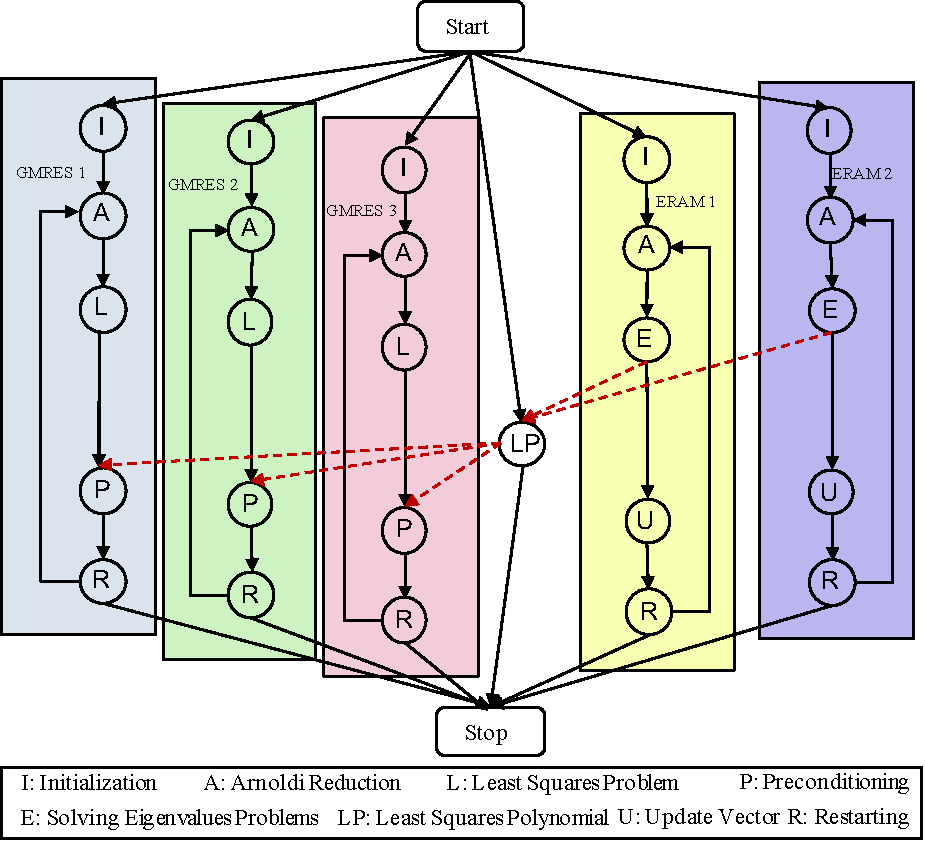
\includegraphics[width=0.8\linewidth]{fig/m-UCGLE-task2.pdf}
	\caption{m-UCGLE task.}
	\label{m-UCGLE-task}
\end{figure}

\subsection{Asynchronous Communications}

The first limitation of YML framework for UC approach is that it does not support the special asynchronous communications (shown as the red dashed arrows in Fig. \ref{m-UCGLE-task}) for the three operations \textit{bgmres\_precond}, \textit{ks\_eigen} and \textit{lsp\_pretreatment}. They send and receive the eigenvalues asynchronously and preconditioning parameters between different computing components. In details, this type of operations can be summarized as: 

\begin{itemize}
	\item check the receiving of data asynchronously from other components; 
	\item if received, operate with these data; if not, perform another operation without these data.
\end{itemize}

\subsection{Mechanism for Convergence}

The second limitation of YML framework for UC approach is the lack of a mechanism to check the convergence of iterative methods. In details, for the GMRES components in Fig. \ref{m-UCGLE-task}, they all perform the loop of Arnoldi reduction until the convergence criteria are satisfied or they exceeded the maximum number of iterations allowed. YML does not allow the mechanism to break the loop in halfway with some given condition. The iterative methods can only be implemented with a fixed number of iterative steps. This kind of implementations is inefficient for the iterative methods, and the convergence cannot always be guaranteed. In the acutal implementation of YML, it is not possible to exit the parallel section/loop of multiple operations until all of them are finished. 

%For the implementation of iterative methods, user give a maximum iteration steps for checking convergence. If the convergence criteria is satisfied, the execution will be stopped before reaching the maximum number of iteration steps. If the convergence can not be achieved even with the maximum number of iterations, the execution will also exit.

\section{Proposition of Solutions}

We reviewed the grammar and scheduler implementations of YML framework, and propose the solution of its limitations for UC approach discussed in Section \ref{Limitations of YML for UC Approach}.

\subsection{Dynamic Graph Grammar in YML}

The special asynchronous communications of UC approach be expressed with extending YML grammar to support the dynamic graphs.

\subsubsection{Variable for Dynamic Graph}\label{Variable for Dynamic Graph}

The dynamic graphs are the types of graph modifiable depends on the variables and/conditions. The dynamic graph can be supported with the introduction of a new variable for the dynamic graph in the \textit{Abstract} components:

\vspace{0.2in}
\begin{minted}
[
frame=lines,
framesep=2mm,
baselinestretch=1.2,
bgcolor=gray!10,
%fontsize=\footnotesize,
%linenos
escapeinside=!!
]
	{xml}
<param type="var_graph" mode="inout" name="foo">
\end{minted}
\vspace{0.2in}

The variable for the dynamic graph can be the mode of \textit{in}, \textit{out} or \textit{inout}. These parameter may be evaluated and modified inside a task, or only as logical into Yvette “if (logical) then $\cdots$ else $\cdots$".

\subsubsection{Scheduler Component for Dynamic Graph}

If the computation to evaluate the logical is too complex, we may use a task with a special indication, added on the Implementation component, such as “graph\_scheduler\_evaluation”: then the scheduler may manage those tasks as others, or run it “itself”.

\subsubsection{Implementation for $m$-UCGLE}

For the implementation of asynchronous communication, it is enough for creating variables to manage the dynamic grammar.  In this section, we give the templates to implement the three computational components:  \textit{bgmres\_precond}, \textit{ks\_eigen} and \textit{lsp\_pretreatment}. This is only an example to show the implementation of variables and the related logic inside the components, so no further detailed information is given. For the rest components without asynchronous dependencies, they can be normally implemented by YML, and we have no intention to give the details in this section.

\textbf{Abstract:} three types of \textit{Abstract} components are constructed as the codes below.  In \textit{ks\_eigen} (shown as Listing \ref{kseigen}), a dynamic graph variable \textit{eigen} is created with the mode "out". In \textit{lsp\_pretreatment} (shown as Listing \ref{lsptreatment}), a dynamic graph variable \textit{lp} is created with the mode "out", and another variable \textit{eigen} is also created with the mode "in". In \textit{bgmres\_precond} (shown as Listing \ref{bgmresprecond}), a dynamic graph variable \textit{lp} is also created with the mode "inout".

\begin{listing}
\begin{minted}
[
frame=lines,
framesep=2mm,
baselinestretch=1.2,
bgcolor=gray!10,
%fontsize=\footnotesize,
%linenos
escapeinside=!!
]
	{xml}
<?xml version="1.0" encoding="utf-8"?>
<component type="abstract" name="ks_eigen_abstract"
description="Eigensolver">
... //defintion of other parameters
<param type="vector_complex" mode="out" name="eigenvalues" /> 
<param type="var_graph" mode="out" name="eigen" />
</component>
\end{minted}
\caption{\textit{ks\_eigen Abstract Component} Implementation}
\label{kseigen}
\end{listing}

\begin{listing}
\begin{minted}
[
frame=lines,
framesep=2mm,
baselinestretch=1.2,
bgcolor=gray!10,
%fontsize=\footnotesize,
%linenos
escapeinside=!!
]
	{xml}
<?xml version="1.0" encoding="utf-8"?>
<component type="abstract" name="lsp_pretreatment_abstract"
description="Least Square Pretreatement">
... //defintion of other parameters
<param type="vector_complex" mode="in" name="eigenvalues" /> 
<param type="var_graph" mode="in" name="eigen" />
<param type="var_graph" mode="out" name="lp" />
<param type="vector_real" mode="out" name="lsparams" /> 
</component>
\end{minted}
\caption{\textit{lsp\_pretreatment Abstract Component} Implementation}
\label{lsptreatment}
\end{listing}

\begin{listing}
\begin{minted}
[
frame=lines,
framesep=2mm,
baselinestretch=1.2,
bgcolor=gray!10,
%fontsize=\footnotesize,
%linenos
escapeinside=!!
]
	{xml}
<?xml version="1.0" encoding="utf-8"?>
<component type="abstract" name="bgmres_precond_abstract"
description="Least Square Preconditioning">
... //defintion of other parameters
<param type="vector_real" mode="in" name="lsparams" /> 
<param type="var_graph" mode="in" name="lp" /> 
<param type="vector_complex" mode="inout" name="residual" /> 
</component>
\end{minted}
\caption{\textit{bgmres\_precond Abstract Component} Implementation}
\label{bgmresprecond}
\end{listing}

\textbf{Implementation:} three \textit{Implementation} components are respetively constructed as Listing \ref{kseigenimpl}, \ref{lsptreatmentimp} and \ref{bgmresprecondimpl} .  We only give the logic inside each component to manage the dynamic graphs.  In \textit{ks\_eigen}, a eigenvalue problem is solved by LAPACK functions. If enough eigenvalues are approximated, the dynamic graph variable will be set as "true", if not, it will be as "false". This variable is output into \textit{lsp\_pretreatment}. In \textit{lsp\_pretreatment}, if the input dynamic graph variable \textit{eigen} is "true",  LS pretreatment operation is executed generate the array \textit{lsparams}, and \textit{lp} is set to be "true". The dynamic graph variable in \textit{bgmres\_precond} is \textit{lp} input from \textit{lsp\_pretreatment}. If this variable is true, a new LS preconditioning residual will be generated using \textit{lsparams}.

\begin{listing}
\begin{minted}
[
frame=lines,
framesep=2mm,
baselinestretch=1.2,
bgcolor=gray!10,
%fontsize=\footnotesize,
%linenos
escapeinside=!!
]
	{xml}
<?xml version="1.0" encoding="utf-8"?>
<component type="impl" name="ks_eigen_impl" description="Eigensolver">
<impl lang="CXX" libs="">
<header><![CDATA[ ]] ></header>
<source lang="CXX" libs="">
</source>
/*solving eigenvalue problem in sequence*/
eigen = false;
eigensolver(&eigenvalues); 
if (enough eignevalues){
	eigen = true;
}
<footer></footer>
</impl>
</component>
\end{minted}
\caption{\textit{ks\_eigen Implementation Component} Implementation}
\label{kseigenimpl}
\end{listing}

\begin{listing}
\begin{minted}
[
frame=lines,
framesep=2mm,
baselinestretch=1.2,
bgcolor=gray!10,
%fontsize=\footnotesize,
%linenos
escapeinside=!!
]
	{xml}
<?xml version="1.0" encoding="utf-8"?>
<component type="impl" name="lsp_pretreatment_impl" description="LP">
<impl lang="CXX" libs="">
<header><![CDATA[ ]] ></header>
<source lang="CXX" libs="">
</source>
 lp = false;
/*generating LS parameters if the eigenvalues available*/
if(eigen){
	LS_Pretreatement(eigenvalues, &lsparams); 
	lp = true;
}
<footer></footer>
</impl>
</component>
\end{minted}
\caption{\textit{lsp\_pretreatment Implementation Component} Implementation}
\label{lsptreatmentimp}
\end{listing}

\begin{listing}
\begin{minted}
[
frame=lines,
framesep=2mm,
baselinestretch=1.2,
bgcolor=gray!10,
%fontsize=\footnotesize,
%linenos
escapeinside=!!
]
	{xml}
<?xml version="1.0" encoding="utf-8"?>
<component type="impl" name="bgmres_precond_impl"
description="LP Preconditioning">
<impl lang="CXX" libs="">
<header><![CDATA[ ]] ></header>
<source lang="CXX" libs="">
</source>
if(lp){
	/*updating LS residual by lsparams*/
	residual=lspreconditioning(lsparams);
}
<footer></footer>
</impl>
</component>
\end{minted}
\caption{\textit{bgmres\_precond Implementation Component} Implementation}
\label{bgmresprecondimpl}
\end{listing}

\begin{figure*}[t]
	\centering
	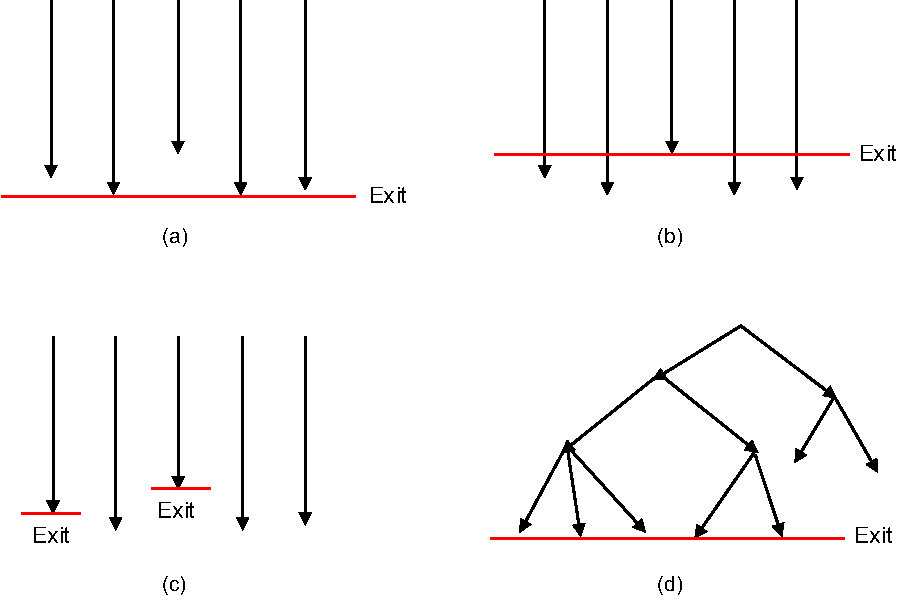
\includegraphics[width=0.9\linewidth]{fig/exit.pdf}
	\caption{Exiting Parallel Branch.}
	\label{fig:exit}
\end{figure*}


\subsection{Exiting Parallel Branch}

The implementation of Exiting parallel branch needs the optimization of scheduler.  In this section, we propose novel implementation of YML scheduler and the related policies for different types of exiting parallel branch.

\subsubsection{Different Types of Exiting Parallel Branch}

In YML, it provides the parallel section and loop, which are able to define explicitly the sections and tasks to be executed in parallel. Inside $m$-UCGLE, the 1st level parallel sections are the different types of computational components, including BGMRES, $s$-KS, and LP. For each parallel section, a number of tasks can be also executed in parallel, e.g., for a number of BGMRES components can be generated in parallel to solve the linear systems with a subset of RHSs, that is the 2nd level of parallel sections inside $m$-UCGLE. Inside each 2nd level task, a series sub-tasks are executed in sequence. For the example of restarted iterative methods with YML, a mechanism for checking the convergence should be established which allows the exiting of parallel section if some conditions are satisfied.  In practice, different modes to exit a parallel branch are required, as shown by Fig. \ref{fig:exit}. Here we list these modes as below:

\begin{enumerate}[label=(\arabic*)]
	\item the application may exit the parallel branch if all the running tasks are completed (shown as Fig. \ref{fig:exit}\textcolor{blue}{a}), e.g., if there are several BGMRES components in parallel to solve linear systems, this parallel section should be exit if all the BGMRES component achieve the convergence;
	\item the application may exit the parallel branch if only one task among all are completed (shown as Fig. \ref{fig:exit}\textcolor{blue}{b}), e.g., in the MERAM algorithm, several ERAM components are executed in parallel to approximate the eigenvalues of a matrix, if one of these components approximates enough eigenvalues, the whole parallel section should be exited;
	\item the application may exit the parallel branch if only several tasks among all are completed (shown as Fig. \ref{fig:exit}\textcolor{blue}{c});
	\item for the application with multi-level parallelism, we may decide to exit several levels of parallelism, (shown as Fig. \ref{fig:exit}\textcolor{blue}{d}, which has three levels of the parallel branch);
	\item the application may exit with the save of selected data into the local filesystems, which will improve its fault tolerance and reusability, e.g., $lsparams$ generated by the LSP Component should be saved into local, which will be used for solving the linear systems in future.
\end{enumerate}

\subsubsection{Optimization of YML Scheduler}

In order to handle the mechanism to exit the parallel branch, a \textit{Exit} feature for YvetteML should be implemented to support the different modes of exiting a parallel branch:

\begin{enumerate}[label=(\arabic*)]
	\item \textit{exit(complete=all)}: all the running tasks of the level are finished before to exit;
	\item \textit{exit(level=p,auto)}: we add to each abstract components if the task has to be finished, data saved or not, we exit the parallel branch ( </exit finish = “yes” />) ; 
	\item \textit{exit(level=p)}: we exit $p$ levels of parallelism ($p$ loops if it is parallel loops);
	\item  we can also add a "save\_exit" type in the asbtract component for the selected parameter as <param type="real" mode="inout" name="A" save\_exit="yes"/>. This parameter will be saved into local file before exiting the branch.
\end{enumerate}

The different types defined above can be used together, which introduces the more flexible logic. 

\begin{enumerate}[label=(\arabic*)]
	\item \textit{exit(complete=all, auto)}: all the running tasks of the level are finished before to exit, except the tasks defined with ( </exit finish = “no” />);
	\item \textit{exit(complete=all, level=p)}: we exit $p$ levels of parallelism if all the tasks in this level are finished;
\end{enumerate}

It is necessary to optimize the YML scheduler policies to support the \textit{exit} grammar. Algorithm \ref{alg:yml-scheduler-op} gives the YML scheduler optimization. The scheduler algorithm is modified as shown by Algorithm \ref{alg:yml-scheduler}. For each task in the parallel branch, its execution status is frequently updated to the scheduler. The scheduler will generate different rules depending on the exit type defined by the YvetteML grammar. This generated exiting rule will be updated to all the tasks managed by this scheduler. This task will be determined to exit or not according to this rule.

\begin{algorithm}[htbp]{}
	\caption{YML Scheduler Optimization}   
	\label{alg:yml-scheduler-op}   
	\begin{algorithmic}[1]
		\While {\textit{status} == EXECUTING}
		\While {\textit{task} == \textit{finished}}
		\State ++\textit{taskFinished}
		\EndWhile
		\State \textcolor{black}{\textit{UpdateStatus}} 
		\State \textcolor{black}{\textit{UpdateSchedulingRuleForExiting}}
		\If {\textcolor{black}{\textit{SchedulingRuleForExiting == true}}}
		\State \textcolor{black}{delete(\textit{task})}
		\EndIf
		\State \textit{UpdateStatus}
		\If{\textit{status}==ERROR}
		\State continue \Comment{Task terminates with error, execution stopped}
		\EndIf 
		\State \textit{UpdateSchedulingRule}
		\While {(\textit{task} = \textit{nextTaskReady}) !=0}
		\State ++\textit{taskSubmitted}
		\State \textit{queue(task)}
		\EndWhile
		\If {!\textit{SchedulingPendingTask}}
		\State break \Comment{Execution finished with error}
		\EndIf
		\State \textit{updateStatus}
		\EndWhile
		\State \textit{finalizExecution}
	\end{algorithmic}  
\end{algorithm}

For the parallel branch with multiple BGMRES components, they will be exited when all the tasks in this parallel level are finished. For the $s$-KS and LSP components, their tasks will be exited if only all the BGMRES components are finished, and they also keep the eigenvalues and \textit{lsparams} into local filesystems, respectively. We give the tentative graph implementation of $m$-UCGLE with the \textit{exit} feature in Listing \ref{uclge-yml}. In this implementation, for the level 2 of the parallel branch with various BGMRES components executing at the same time, we add \textit{exit(complete=all)}. This means that these BGMRES tasks should be exited until all the tasks are completed with all BGMRES components achieving the convergence. For the tasks of LSP and $s$-KS components, they should be exited only if all the tasks of BGMRES are finished. Thus in the implementation of their \textit{Abstract Components}, we add the parameter (</exit finish = "no">), which means these tasks need not be finished before exiting. In the \textit{Abstract Components} of \textit{ks\_eigen}, the definition of the parameter \textit{eigenvalues} is modified to be <param type="vector\_complex" mode="out" name="eigenvalues" save\_exit="yes"/>, which means that the approximated eigenvalues should be saved into local file before exiting. Similarly,  the parameter \textit{lsparams} should also be saved, and its definition is  changed to be <param type="vector\_real" mode="out" name="lsparams" save\_exit="yes"/>. In order to exit the parallel branch of level 1 which express the parallel execution of BGMRES, LSP and $s$-KS, we add \textit{exit(complete=all, auto)}. In this level of the parallel branch, the tasks will be executed until all the tasks are finished, except the tasks are defined with (</exit finish = "no">). Hence the logic is: if all the tasks in level 2 of the parallel branch of BGMRES are finished, they will exit this level of the branch. For the branch of level 1, all the tasks completed means the finish of all tasks of BGMRES, thus, if all the BGMRES obtain the convergence, they will exit the level 2, and then immediately exit the level 1, and $m$-UCGLE is exit. 

\section{Demand for MPI Correction Mechanism}

For the multi-level parallel programming paradigm YML/XMP, it is necessary to investigate the application of scalable correctness checking methods to YML, XMP and selected features of MPI. This will result in a clear guideline how to limit the risk to introduce errors and how to best express the parallelism to catch errors that for principle reasons can only be detected at runtime, as well as extended and scalable correctness checking methods.

MUST\footnote{https://tu-dresden.de/zih/forschung/projekte/must} detects usage errors of the Message Passing Interface (MPI) and reports them to the user. As MPI calls are complex and usage errors common, this functionality is extremely helpful for application developers that want to develop correct MPI applications. To detect errors, MUST intercepts the MPI calls that are issued by the target application and evaluates their arguments. The two main usage scenarios for MUST arise during application development and when porting an existing application to a new system. When a developer adds new MPI communication calls, MUST can detect newly introduced errors, especially also some that may not manifest in an application crash. Further, before porting an application to a new system, MUST can detect violations to the MPI standard that might manifest on the target system. MUST reports errors in a log file that can be investigated once the execution of the target executable finishes. On the large-scale computing systems, it is necessary to use MUST as a tool to check all kinds of MPI errors during the whole life cycle of YML/XMP applications.

\begin{listing}
\begin{minted}
[
frame=lines,
framesep=2mm,
baselinestretch=1.2,
bgcolor=gray!10,
%fontsize=\footnotesize,
%linenos
escapeinside=||
]
{xml}
<?xml version="1.0" encoding="utf-8"?>
<application name="dyntest_app">
<description> m-UCGLE prototype </description>
<params></params>
<graph>
ngmres: = 3; neram: = 2;
|\textcolor{red}{par}| |\textcolor{green!60!black}{do}|
	|\textcolor{red}{par}|(gid: = 0; ngmres-1) |\textcolor{green!60!black}{do}|
		|\textcolor{purple}{compute}| bgmres_init(gid, ... );
		|\textcolor{blue!60!black}{seq}|(g_restart: =0; max_restart_nb-1) |\textcolor{green!60!black}{do}|
			|\textcolor{purple}{compute}| bgmres_ar(gid, ... );
			|\textcolor{purple}{compute}| bgmres_ls(gid, ... );
			|\textcolor{purple}{compute}| bgmres_precond(gid, ... );
			|\textcolor{purple}{compute}| bgmres_check(gid, ... );
			|\textcolor{purple}{compute}| bgmres_restart(gid, ... );
			|\textcolor{violet}{exit}|(complete=all);
		|\textcolor{green!60!black}{enddo}|
	|\textcolor{green!60!black}{enddo}| |\textcolor{red}{endpar}|
	|\textcolor{red}{par}|(eid: = ngmres; ngmres+neram-1) |\textcolor{green!60!black}{do}|
	    |\textcolor{purple}{compute}| ks_init(eid, ... );
		|\textcolor{blue!60!black}{seq}|(e_restart: =0; max_restart_nb-1) |\textcolor{green!60!black}{do}|
			|\textcolor{purple}{compute}| ks_ar(eid, ... );
			|\textcolor{purple}{compute}| ks_eigen(eid, ... );
			|\textcolor{purple}{compute}| ks_update(eid, ... );
			|\textcolor{purple}{compute}| ks_restart(eid, ... );
		|\textcolor{green!60!black}{enddo}|
	|\textcolor{green!60!black}{enddo}| |\textcolor{green!60!black}{do}|
	|\textcolor{purple}{compute}| lsp_pretreatment(ngmres+neram, ... );
	|\textcolor{violet}{exit}|(complete=all, auto); 
|\textcolor{green!60!black}{enddo}| |\textcolor{red}{endpar}|
</graph>
</application>
\end{minted}
\caption{Tentaive implememtation of $m$-UCGLE's graph}
\label{uclge-yml}
\end{listing}

\section{Conclusion}

In this chapter, we investigate the prossibility to implement the iterative methods based on UC approach using the YML workflow runtime. There are two limitations of current implementation: 1) asynchronous communication between the computational components; 2) exit the parallel branch. We propose the solution by adding variable to handle the dynamic graphs, and optimize the scheduler rules to manage different modes of exiting parallel branches. These proposed solution should be embedded into YML in the future.


\clearemptydoublepage

\clearemptydoublepage